\documentclass[11pt,a4paper]{report}

% ---------- Packages ----------
\usepackage[a4paper,margin=1in]{geometry}
\usepackage{graphicx}
\usepackage{xcolor}
\usepackage{tikz}
\usetikzlibrary{shapes.geometric,arrows.meta,positioning,fit,backgrounds}
\usepackage{booktabs}
\usepackage{array}
\usepackage{enumitem}
\usepackage{fancyhdr}
\usepackage{titlesec}
\usepackage{caption}
\usepackage{float}
\usepackage{hyperref}
\usepackage{amsmath}
\usepackage{listings}
\usepackage{longtable}
\usepackage{parskip}

% ---------- Colors ----------
\definecolor{navy}{RGB}{15,17,23}
\definecolor{accentblue}{RGB}{47,111,237}
\definecolor{accentred}{RGB}{233,69,96}
\definecolor{accentgreen}{RGB}{34,197,94}
\definecolor{lightgray}{RGB}{245,245,247}
\definecolor{codebg}{RGB}{247,247,250}

\hypersetup{
  colorlinks=true,
  linkcolor=accentblue,
  citecolor=accentblue,
  urlcolor=accentblue,
  pdftitle={Phishing Simulation, Awareness Training and ML/DL-Based URL Detection},
  pdfauthor={Ayush Gupta}
}

% ---------- Header/Footer ----------
\pagestyle{fancy}
\fancyhf{}
\renewcommand{\headrulewidth}{0.4pt}
\fancyhead[L]{\small\itshape Phishing Simulation \& Detection}
\fancyhead[R]{\small\itshape Chapter \thechapter}
\fancyfoot[C]{\thepage}

% ---------- Section styling ----------
\titleformat{\chapter}[display]
  {\normalfont\huge\bfseries\color{navy}}
  {\chaptertitlename\ \thechapter}{20pt}{\Huge}
\titleformat{\section}
  {\normalfont\Large\bfseries\color{accentblue}}
  {\thesection}{1em}{}
\titleformat{\subsection}
  {\normalfont\large\bfseries}
  {\thesubsection}{1em}{}

\lstset{
  backgroundcolor=\color{codebg},
  basicstyle=\ttfamily\footnotesize,
  frame=single,
  breaklines=true,
  columns=fullflexible,
  rulecolor=\color{gray!40}
}

\newcommand{\screenshot}[3]{%
  \begin{figure}[H]
    \centering
    \includegraphics[width=#2\textwidth]{screenshots/#1}
    \caption{#3}
  \end{figure}
}

\title{
  \vspace{-2cm}
  {\Huge\bfseries Phishing Simulation, Security Awareness Training\\[6pt] and ML/DL-Based Phishing URL Detection}\\[1cm]
  {\large A Two-Part Cybersecurity Project Report}
}
\author{Ayush Gupta}
\date{July 2026}

\begin{document}

\begin{titlepage}
\centering
\vspace*{2cm}
{\Huge\bfseries Phishing Simulation, Security\\[4pt] Awareness Training and\\[4pt] ML/DL-Based Phishing URL Detection\par}
\vspace{1cm}
{\Large A Two-Part Cybersecurity Project Report\par}
\vspace{2cm}

{\large\itshape
Part I: Simulated phishing campaigns (clone login page, malicious-attachment\\
simulation, QR-code/OTP simulation) built for internal security awareness training.\\[8pt]
Part II: A hybrid machine-learning / deep-learning pipeline for automated\\
phishing URL detection.\par}

\vfill

\begin{center}
\begin{tabular}{ll}
\textbf{Author:} & Ayush Gupta \\
\textbf{Date:} & July 2026 \\
\end{tabular}
\end{center}

\vspace{1cm}
{\small\itshape
All simulated phishing pages in this project display an explicit ``this was a\\
phishing simulation'' disclosure after interaction and store no real credentials\\
or personal data. They are intended solely for authorized, internal security\\
awareness training.\par}

\end{titlepage}

\tableofcontents
\listoffigures
\clearpage

% ======================================================================
\part{Phishing Simulation and Security Awareness Training}
% ======================================================================

\chapter{Introduction and Vision}

\section{Motivation}
Phishing remains the single most common initial-access technique used in cyberattacks:
rather than breaking cryptography or exploiting a zero-day vulnerability, an attacker
simply asks the victim to hand over credentials, install malware, or approve a
fraudulent transaction --- and dresses the request up as something routine and
trustworthy. Because the weakest link is human judgement rather than a technical
control, the most effective defense is not a firewall rule but \emph{trained
suspicion}: employees who have already seen what a convincing phishing attempt looks
like, in a safe setting, are measurably less likely to fall for a real one.

This project has two complementary halves that both attack this same problem from
opposite ends:

\begin{itemize}[leftmargin=1.4em]
  \item \textbf{Part I -- Offense-as-training.} A small set of realistic, self-contained
  phishing simulations (a cloned Microsoft login page, a disguised malicious
  attachment, and a QR-code/OTP reward scam) that can be sent to employees exactly as
  a real attacker would send them. Each simulation captures whether the target fell
  for it, and --- critically --- immediately reveals itself as a training exercise and
  explains what real-world red flags were present, turning a moment of embarrassment
  into a teachable moment.
  \item \textbf{Part II -- Defense via automation.} A machine-learning system that
  classifies arbitrary URLs as phishing or legitimate in real time, so that even
  attempts nobody has been specifically trained against can be caught before a human
  has to make the judgement call at all.
\end{itemize}

\section{Ethical and Operational Boundaries}
Every simulation in this project is built around three non-negotiable rules:

\begin{enumerate}[leftmargin=1.4em]
  \item \textbf{No real credentials or personal data are ever stored.} Login forms,
  OTP entry, and file execution are all purely client-side theater --- nothing typed
  into them is transmitted to any credential store or third party.
  \item \textbf{Immediate, unambiguous self-disclosure.} The instant a target
  completes the simulated action (submits a password, enters an OTP, opens the fake
  attachment), the page reveals itself as a security-awareness exercise and explains
  the real-world warning signs the target should have noticed.
  \item \textbf{Authorized, internal use only.} These simulations are designed to be
  run by an organization against its own employees (or by an individual against
  consenting test subjects), analogous to commercial phishing-simulation products
  used by corporate security teams -- never against the public or without consent.
\end{enumerate}

\chapter{Background: What is Phishing?}

\section{Definition}
Phishing is a social-engineering attack in which an adversary impersonates a
trustworthy entity --- a company, colleague, government agency, or well-known brand
--- in order to trick a victim into revealing sensitive information (passwords, OTPs,
credit-card numbers), installing malicious software, or performing an action that
benefits the attacker (e.g.\ wiring money). The term is a homophone of ``fishing'':
the attacker casts a baited hook (a convincing message) and waits for a victim to
bite.

\section{Common Categories of Phishing}
Phishing is not a single technique but a family of related attacks that differ in
delivery channel, targeting precision, and payload. The categories most relevant to
this project are summarized below.

\begin{longtable}{@{}p{3.3cm}p{11.5cm}@{}}
\toprule
\textbf{Type} & \textbf{Description} \\
\midrule
\endhead
Email phishing & Mass, untargeted fraudulent emails impersonating a bank, vendor, or
service, urging the recipient to click a link or open an attachment. The oldest and
still most common phishing vector. \\[4pt]
Spear phishing & A targeted variant aimed at a specific individual or organization,
using personal details (name, role, recent activity) to increase credibility. \\[4pt]
Whaling & Spear phishing aimed specifically at senior executives or other
high-value targets, often impersonating a CEO or board member. \\[4pt]
Clone phishing & An attacker copies a legitimate, previously-seen email or website
almost exactly, replacing a link or attachment with a malicious one. \emph{This
project's Microsoft login clone is a clone-phishing simulation.} \\[4pt]
Smishing & Phishing delivered via SMS text message, typically containing a
shortened or disguised link. \\[4pt]
Vishing & Voice phishing conducted over a phone call, often impersonating tech
support, a bank's fraud department, or a government agency. \\[4pt]
Quishing (QR-code phishing) & A malicious URL is embedded in a QR code rather than a
clickable link, exploiting the fact that a scanned QR code's destination is not
visible before the phone's browser opens it. \emph{This project's QR/OTP reward
simulation is a quishing simulation.} \\[4pt]
Malicious-attachment phishing & The email's payload is a disguised executable or
macro-laden document rather than a credential-harvesting link; opening it installs
malware directly. \emph{This project's ``HiApp'' fake-PDF simulation demonstrates
this technique.} \\[4pt]
Pharming & DNS or hosts-file manipulation redirects a victim from a legitimate
domain to a fraudulent one even when they type the correct address. \\[4pt]
Business Email Compromise (BEC) & An attacker compromises or spoofs a real
corporate email account to authorize fraudulent wire transfers or data disclosure,
typically without any malicious link at all. \\
\bottomrule
\end{longtable}

\section{Why Simulation-Based Training Works}
Studies of enterprise security programs consistently find that periodic, realistic
phishing simulations --- paired with immediate, specific feedback at the moment of
failure --- reduce click-through rates on subsequent real phishing attempts far more
effectively than annual slideshow training alone. The mechanism is simple: reading
about phishing is abstract, but nearly entering your own password into a fake
Microsoft login page and then being told exactly which visual and technical cues gave
it away creates a memorable, specific mental model of what to look for next time.
This is the design principle behind every simulation in Part I of this project.

\chapter{Simulation 1: Clone Phishing -- Fake Microsoft Login Page}

\section{Attack Scenario}
The simulated campaign begins with an email sent to the target employee, styled as an
automated IT notice warning that their Microsoft 365 password is about to expire and
urging them to click a \emph{Reset Password} link before a same-day deadline --
a deliberately mild urgency cue (a looming deadline, framed as routine IT
housekeeping) chosen because it is far more effective at suppressing suspicion than
an alarming one.

\screenshot{ms_login_0_pretext_email.png}{0.85}{The pretext email as it lands in the target's inbox: a spoofed sender name and address (\texttt{microsot\_suppor@outlook.com} -- note the misspelling), a fabricated password-expiration notice with a same-day deadline, and a \emph{Reset Password} link. Gmail's own spam filter already flagged it as suspicious, illustrating that even a fairly crude pretext can still reach and fool a recipient who does not stop to check the sender address or the filter's warning.}

The \emph{Reset Password} link is the payload: it points not to a real Microsoft
domain but to the locally-hosted clone of the Microsoft/Outlook sign-in page
described below. Because the destination page is visually indistinguishable from
the real thing, an employee who clicks through without checking the address bar will
often proceed straight through the sign-in flow exactly as they would on the genuine
site.

\section{Page Flow}
The clone reproduces Microsoft's real two-step sign-in flow (email, then password) as
a single-page application with three view states, and only reveals the training
disclosure after both steps are completed -- mirroring the real attack sequence a
credential-harvesting kit would use.

\screenshot{ms_login_1_email.png}{0.62}{Stage 1 -- where the \emph{Reset Password} link lands: the cloned Microsoft sign-in page, requesting an email/phone/Skype identifier. Visually matches the real Microsoft sign-in page's layout, logo, and typography.}

\screenshot{ms_login_2_password.png}{0.62}{Stage 2 -- after entering an identifier, the clone advances to a password prompt, echoing the identifier back exactly as the real flow does.}

\screenshot{ms_login_3_awareness.png}{0.62}{Stage 3 -- immediately after ``signing in,'' the page reveals itself as a phishing simulation and lists the concrete red flags the target should check next time (address bar URL, unsolicited re-authentication requests, reporting channel).}

\section{Technical Implementation}
\begin{itemize}[leftmargin=1.4em]
  \item \textbf{Stack:} static HTML/CSS/JavaScript, no backend dependency for the
  page itself.
  \item \textbf{State machine:} three \texttt{<section>} blocks
  (\texttt{section\_uname}, \texttt{section\_pwd}, \texttt{section\_final}) toggled
  via a \texttt{d-none} CSS class, driven by \texttt{app.js}.
  \item \textbf{No credential capture:} the password field's value is read only to
  gate the transition to the disclosure screen -- it is never transmitted or written
  to storage.
  \item \textbf{Telemetry:} on page load and on credential submission, a
  fire-and-forget \texttt{fetch()} call posts an anonymous event
  (\texttt{page\_view} / \texttt{credential\_submit}) to the central tracking
  dashboard described in Chapter~5, tagged with campaign id \texttt{ms-login}.
\end{itemize}

\chapter{Simulation 2: Malicious Attachment Disguised as a PDF (``HiApp'')}

\section{Attack Scenario}
The pretext email reads:

\begin{quote}\itshape
``Please review the attached document urgently and confirm before end of day.''
\end{quote}

The attachment appears to be a PDF, but is in fact a packaged executable
(\texttt{HiApp.exe}, built with Electron). This mirrors one of the oldest and still
most effective malware-delivery techniques: disguising an executable's true file type
using a deceptive filename, icon, or double extension so that a rushed employee opens
it without checking the real extension.

\section{Behavior}
On launch, the program immediately displays a full-screen disclosure -- there is no
hidden payload beyond this message, since the program's sole purpose is the training
exercise itself.

\screenshot{hiapp_awareness.png}{0.62}{HiApp's disclosure screen, shown immediately on launch: it explains that the ``PDF'' was actually an executable, and that in a real attack this exact confusion is how malware gets installed.}

\section{Technical Implementation}
\begin{itemize}[leftmargin=1.4em]
  \item \textbf{Stack:} Electron (\texttt{main.js} creates a single
  \texttt{BrowserWindow} loading a local \texttt{index.html}), packaged for Windows
  via \texttt{electron-builder} with a one-click NSIS installer profile.
  \item \textbf{Deceptive delivery (simulated):} in a real campaign this binary would
  be renamed/iconed to resemble a PDF attachment; the underlying Electron app itself
  is harmless and performs no filesystem or network action beyond the training
  disclosure.
  \item \textbf{Telemetry:} on launch, an \texttt{exe\_run} event is posted to the
  dashboard under campaign id \texttt{exe}.
\end{itemize}

\chapter{Simulation 3: QR Code / OTP Phishing (``Claim Your Reward'')}

\section{Attack Scenario}
The target receives a QR code (e.g.\ printed on a flyer, or emailed as an image)
captioned ``Scan to claim your reward.'' Scanning it with a phone camera opens a
mobile-styled page asking for a 6-digit OTP. This simulates a real and increasingly
common attack pattern (\emph{quishing}): the attacker relies on the fact that a
scanned QR code's destination URL is largely invisible to the user before their
browser navigates to it, and pairs it with the classic pretext of an unexpected
reward to short-circuit suspicion. In a real attack this OTP would be the
one-time code from the victim's actual bank or email account, harvested in real time
to complete an account-takeover elsewhere.

\screenshot{rewards_1_otp_form.png}{0.55}{The QR-code landing page: a ``Claim Your Reward'' prompt asking the target to enter a 6-digit OTP, styled to feel casual and low-stakes.}

\screenshot{rewards_2_awareness.png}{0.55}{Immediately after submission, the page discloses the simulation and gives the specific rule the target should internalize: never enter a real OTP on a page reached via an unverified QR code.}

\section{Technical Implementation}
\begin{itemize}[leftmargin=1.4em]
  \item \textbf{Stack:} static HTML/CSS/JavaScript, with auto-advancing individual
  OTP digit inputs (focus moves to the next box as each digit is typed, matching the
  UX of real OTP-entry pages so the simulation feels authentic).
  \item \textbf{No OTP capture:} the entered digits are never transmitted or stored;
  they are read only to trigger the transition to the disclosure view.
  \item \textbf{Telemetry:} \texttt{page\_view} and \texttt{otp\_submit} events are
  posted under campaign id \texttt{qr-otp}.
\end{itemize}

\chapter{Centralized Awareness Dashboard}

\section{Purpose}
All three simulations report anonymous, aggregate telemetry to a single dashboard, so
that whoever runs the awareness campaign can measure --- across an entire
organization or test group --- how many people viewed each lure, and how many
actually fell for it (entered a password, entered an OTP, or ran the fake
executable). This is the same measurement loop used by commercial phishing-simulation
platforms: without it, a training exercise cannot demonstrate its own effectiveness.

\section{Architecture}
\begin{itemize}[leftmargin=1.4em]
  \item \textbf{Stack:} Node.js + Express, with events persisted to a flat
  \texttt{events.json} file (sufficient for a single-organization awareness
  exercise; the schema is a simple append-only event log).
  \item \textbf{Endpoints:}
  \begin{itemize}
    \item \texttt{POST /api/event} -- records a \texttt{\{campaign, type\}} event
    along with timestamp, source IP, and user agent.
    \item \texttt{GET /api/stats} -- returns aggregate per-campaign counts and the
    25 most recent events, polled by the dashboard every 4 seconds.
    \item \texttt{POST /api/reset} -- clears all recorded events, gated behind a
    shared secret key.
  \end{itemize}
  \item \textbf{Validation:} both campaign id and event type are checked against a
  fixed allow-list server-side, so malformed or spoofed events cannot pollute the
  dashboard.
\end{itemize}

\begin{figure}[H]
  \centering
  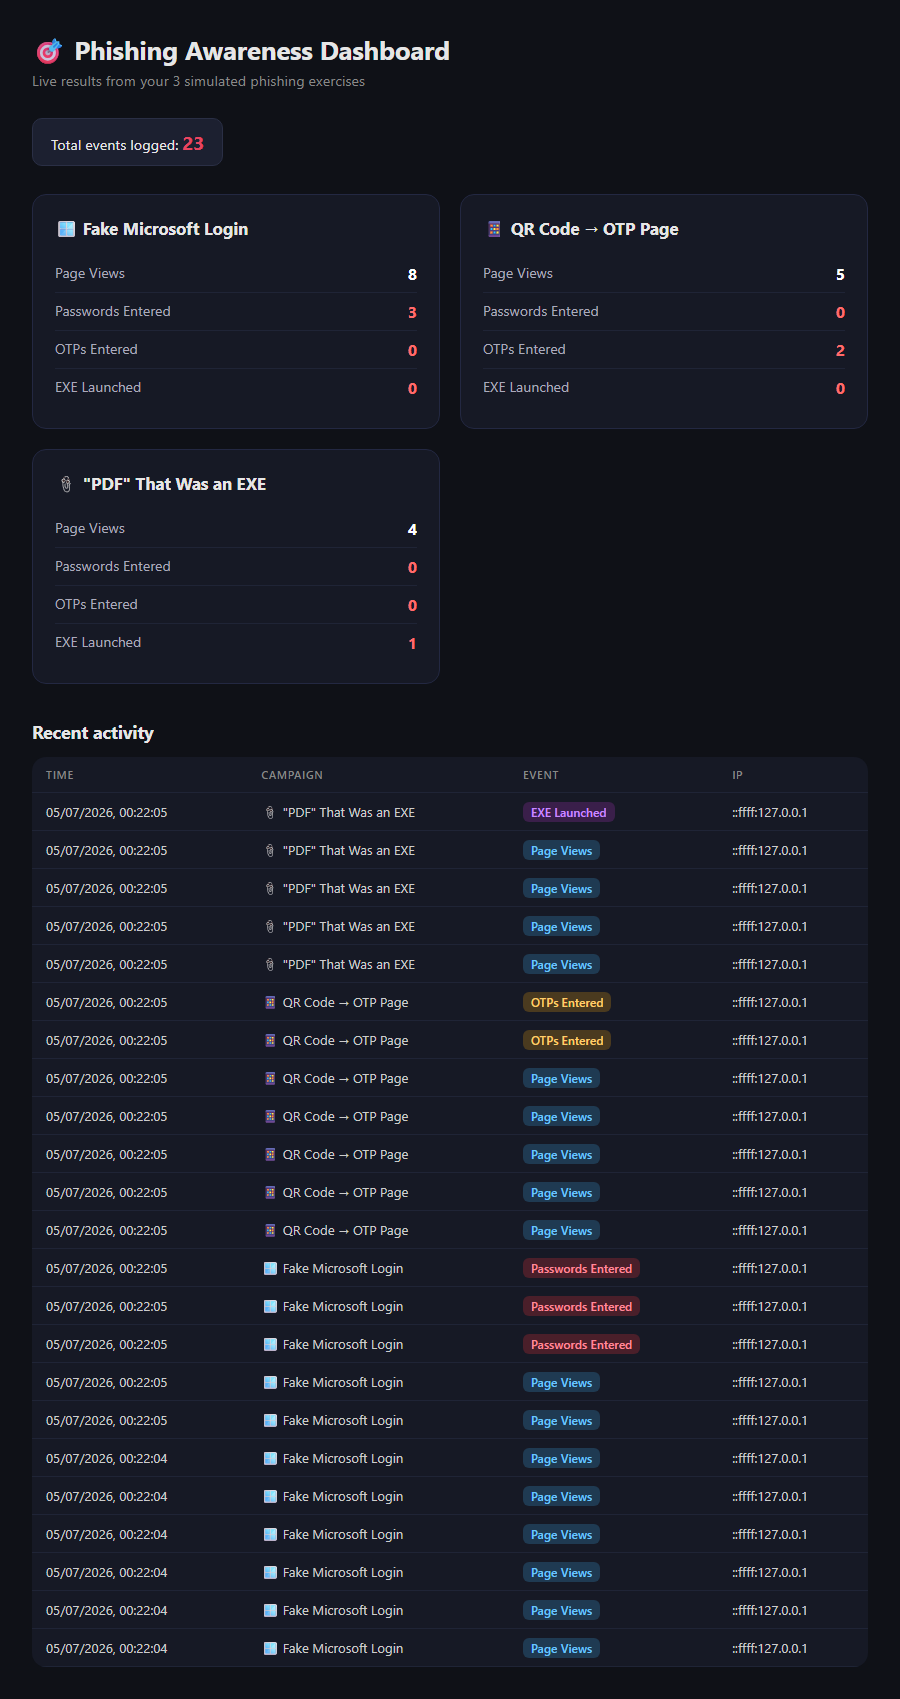
\includegraphics[height=0.82\textheight,keepaspectratio]{screenshots/dashboard.png}
  \caption{The awareness dashboard, showing per-campaign totals (page views vs.\ the ``dangerous'' actions: passwords entered, OTPs entered, EXE launched) and a live recent-activity feed. Data shown here is illustrative sample data generated for this report.}
\end{figure}

\section{Campaign Lifecycle}
Figure~\ref{fig:campaign-flow} summarizes the end-to-end lifecycle common to all
three simulations: an attacker-styled pretext delivered by email or QR code, a
convincing but inert simulated payload, an immediate self-disclosure at the moment
of ``compromise,'' and anonymous telemetry feeding the aggregate dashboard.

\begin{figure}[H]
\centering
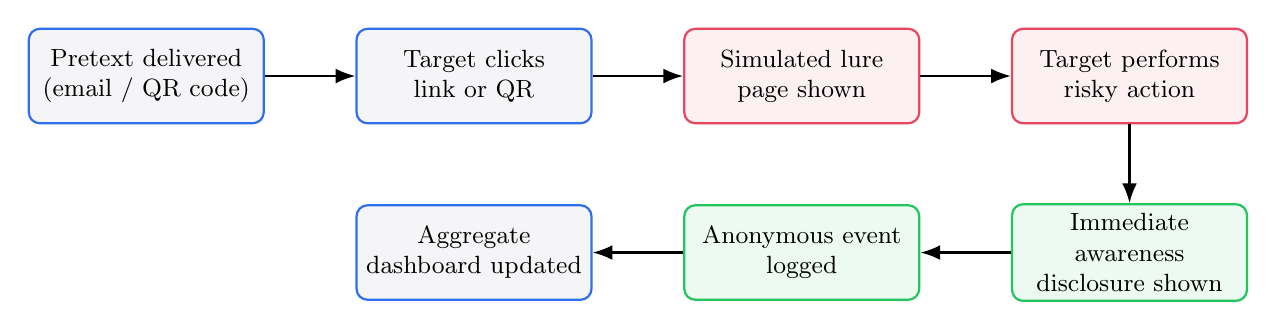
\begin{tikzpicture}[
  node distance=1.0cm and 1.15cm,
  box/.style={rectangle, rounded corners, draw=accentblue, thick, fill=lightgray,
    text width=2.75cm, align=center, minimum height=1.2cm, font=\small},
  danger/.style={box, draw=accentred, fill=accentred!8},
  safe/.style={box, draw=accentgreen, fill=accentgreen!8},
  arr/.style={-{Latex[length=2.5mm]}, thick}
]
\node[box] (email) {Pretext delivered\\(email / QR code)};
\node[box, right=of email] (click) {Target clicks\\link or QR};
\node[danger, right=of click] (lure) {Simulated lure\\page shown};
\node[danger, right=of lure] (action) {Target performs\\risky action};
\node[safe, below=of action] (reveal) {Immediate awareness\\disclosure shown};
\node[safe, left=of reveal] (log) {Anonymous event\\logged};
\node[box, left=of log] (dash) {Aggregate\\dashboard updated};

\draw[arr] (email) -- (click);
\draw[arr] (click) -- (lure);
\draw[arr] (lure) -- (action);
\draw[arr] (action) -- (reveal);
\draw[arr] (reveal) -- (log);
\draw[arr] (log) -- (dash);
\end{tikzpicture}
\caption{End-to-end lifecycle of a single simulated phishing campaign, common to all three simulations in Part I.}
\label{fig:campaign-flow}
\end{figure}

% ======================================================================
\part{ML/DL-Based Phishing URL Detection}
% ======================================================================

\chapter{Motivation and Problem Statement}

\section{Limitations of the Original Approach}
The project began with a conventional phishing-URL classifier: a single
scikit-learn model (RandomForest / GradientBoosting / XGBoost, model-selected by
cross-validated ROC-AUC) trained on a public 30-feature dataset in which most
features required a \emph{live} lookup at prediction time --- a WHOIS query for
domain age, a screen-scraped Google search to check indexing, and calls to two
third-party ranking services (the Alexa traffic-rank API and
\texttt{checkpagerank.net}). In practice this made the classifier fragile in three
concrete ways:

\begin{itemize}[leftmargin=1.4em]
  \item \textbf{Dead dependencies.} The Alexa API was discontinued in 2022, and
  \texttt{checkpagerank.net} no longer serves the expected response --- both features
  silently degrade to a constant value for every URL, contributing noise rather than
  signal.
  \item \textbf{Fragile dependencies.} WHOIS lookups and Google-search scraping are
  rate-limited and frequently blocked outright, meaning classification could fail or
  time out on exactly the live traffic a production system needs to handle.
  \item \textbf{Latency.} Because every prediction required several live network
  round-trips, a single classification could take seconds --- unacceptable for
  inline, real-time URL screening.
\end{itemize}

\section{Design Goals for the New Pipeline}
The rebuilt pipeline was designed around four goals:

\begin{enumerate}[leftmargin=1.4em]
  \item \textbf{Fully offline inference.} Every feature used at prediction time
  must be computable from the URL string alone, in microseconds, with no external
  network call.
  \item \textbf{Combine complementary signal sources.} Hand-engineered features
  encode domain expertise (what a security analyst would look for) but cannot
  anticipate every future obfuscation trick; a learned representation over raw
  characters can pick up patterns no one thought to encode by hand. Using both,
  combined by a trained meta-model rather than a fixed rule, should outperform either
  alone.
  \item \textbf{Train and evaluate on live, current data} rather than a static,
  multi-year-old public dataset whose phishing examples no longer reflect current
  attacker tooling.
  \item \textbf{Guard against the model's own blind spots} with an explicit,
  auditable safeguard rather than relying solely on statistical generalization.
\end{enumerate}

\chapter{System Architecture}

\section{Overview}
The final system is a \textbf{hybrid ensemble} of two independently-trained
classifiers, combined by a logistic-regression meta-model, with a trusted-domain
allow-list applied as a final safeguard. Figure~\ref{fig:architecture} shows the full
inference-time data flow.

\begin{figure}[H]
\centering
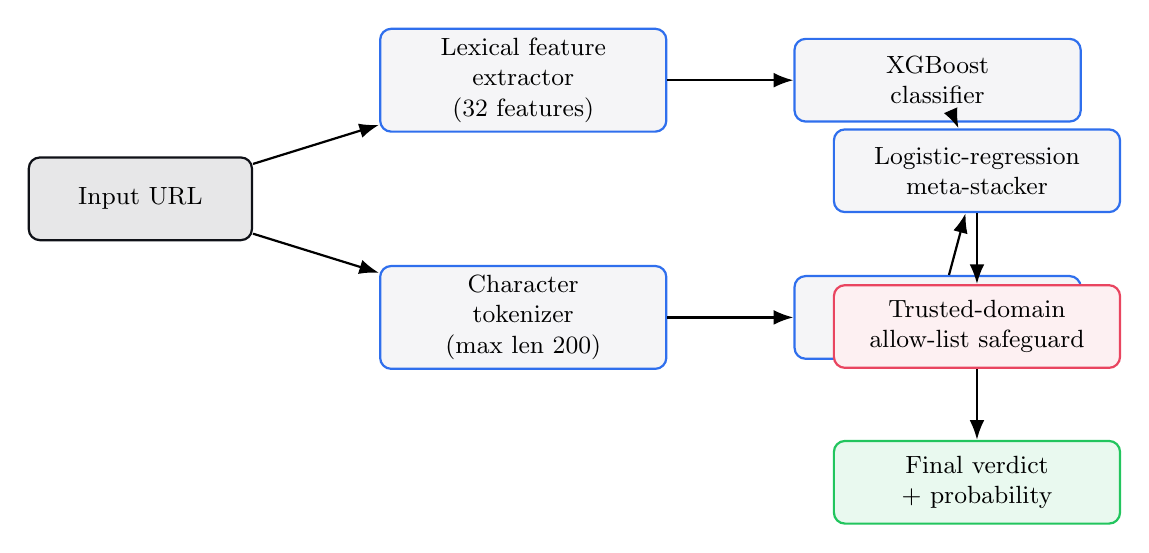
\begin{tikzpicture}[
  node distance=0.9cm and 1.4cm,
  box/.style={rectangle, rounded corners, draw=accentblue, thick, fill=lightgray,
    text width=3.4cm, align=center, minimum height=1.05cm, font=\small},
  urlbox/.style={box, draw=navy, fill=navy!10, text width=2.6cm},
  outbox/.style={box, draw=accentgreen, fill=accentgreen!10, text width=3.4cm},
  arr/.style={-{Latex[length=2.5mm]}, thick}
]
\node[urlbox] (url) {Input URL};
\node[box, above right=0.3cm and 1.6cm of url] (lex) {Lexical feature\\extractor\\(32 features)};
\node[box, below right=0.3cm and 1.6cm of url] (chr) {Character\\tokenizer\\(max len 200)};
\node[box, right=1.6cm of lex] (xgb) {XGBoost\\classifier};
\node[box, right=1.6cm of chr] (cnn) {CharCNN\\(GPU, PyTorch)};
\node[box, right=2.1cm of lex, yshift=-1.15cm] (meta) {Logistic-regression\\meta-stacker};
\node[box, below=0.9cm of meta, draw=accentred, fill=accentred!8] (allow) {Trusted-domain\\allow-list safeguard};
\node[outbox, below=0.9cm of allow] (out) {Final verdict\\+ probability};

\draw[arr] (url) -- (lex);
\draw[arr] (url) -- (chr);
\draw[arr] (lex) -- (xgb);
\draw[arr] (chr) -- (cnn);
\draw[arr] (xgb) -- (meta);
\draw[arr] (cnn) -- (meta);
\draw[arr] (meta) -- (allow);
\draw[arr] (allow) -- (out);
\end{tikzpicture}
\caption{Hybrid pipeline architecture: two independent branches (lexical-feature XGBoost, and character-level CharCNN) are combined by a trained meta-stacker, with a final trusted-domain allow-list safeguard.}
\label{fig:architecture}
\end{figure}

\section{Branch A -- XGBoost over Lexical/Structural Features}
This branch computes 32 numeric features from the URL string alone (implemented in
\url{pipeline/lexical_features.py}), grouped into four families:

\begin{itemize}[leftmargin=1.4em]
  \item \textbf{Length/composition statistics:} URL, hostname, path and query
  length; counts of dots, hyphens, underscores, slashes, digits and special
  characters; digit-to-length ratio.
  \item \textbf{Randomness/obfuscation indicators:} Shannon entropy of the full URL
  and of the hostname alone (machine-generated or algorithmically-obfuscated domains
  tend to look statistically ``noisier'' than human-chosen names); presence of a raw
  IP-address host; presence of an \texttt{@} symbol; suspicious \texttt{//}
  mid-path redirection; punycode (\texttt{xn--}) domains, which can encode
  homograph/look-alike Unicode characters.
  \item \textbf{Brand-impersonation detection:} domain tokens (split on hyphens/
  digits) are compared via Levenshtein edit distance against a curated list of
  frequently-impersonated brand names (PayPal, Microsoft, Apple, major banks, etc.);
  a near-miss token that is \emph{not} an exact match to the real brand domain (e.g.\
  the token \texttt{paypa1} in \texttt{paypa1-secure-login.tk}) is a strong
  typosquatting signal. A separate feature flags a brand name appearing in a
  subdomain while absent from the actual registered domain.
  \item \textbf{Structural/contextual flags:} known-abused top-level domains
  (\texttt{.tk}, \texttt{.xyz}, \texttt{.top}, etc.), known URL-shortener domains,
  HTTPS usage, non-standard ports, subdomain count/depth, path depth, query
  parameter count, and a count of credential/urgency keywords
  (\texttt{login}, \texttt{verify}, \texttt{secure}, \texttt{suspend}, \ldots)
  appearing anywhere in the URL.
\end{itemize}

These features are passed to a gradient-boosted tree ensemble (\texttt{XGBClassifier},
300 trees, max depth 6, learning rate 0.08), with \texttt{scale\_pos\_weight} set to
the training set's negative/positive class ratio to correct for class imbalance.

\section{Branch B -- Character-Level CNN over the Raw URL}
Rather than relying solely on hand-designed features, the second branch
(\url{pipeline/char_model.py}) learns directly from the URL's raw character
sequence, so that sub-word patterns no engineered feature explicitly captures ---
unusual character-substitution patterns, novel token structures, or unseen
typosquat variants --- can still be picked up.

\begin{itemize}[leftmargin=1.4em]
  \item Each URL is lower-cased and encoded as a fixed-length sequence of integer
  character ids (vocabulary of 61 characters covering letters, digits, and common
  URL punctuation; sequences truncated/padded to 200 characters).
  \item A learned character embedding (dimension 32) feeds three parallel 1-D
  convolutions with kernel sizes 3, 5, and 7 (64 filters each), capturing character
  n-gram patterns at multiple scales.
  \item Global max-pooling over each convolution's output is concatenated and passed
  through two fully-connected layers (64 units, then a single logit), with dropout
  (0.3) for regularization.
  \item Trained with the Adam optimizer and binary cross-entropy loss, on an
  NVIDIA GPU (CUDA) for fast iteration --- full training on this dataset converges
  in well under two minutes on a consumer-grade GPU, versus multiple times longer on
  CPU alone.
\end{itemize}

\section{Meta-Stacker -- Combining Both Branches}
Rather than averaging the two branches' predictions with a fixed weight, a
logistic-regression meta-model is trained on their \emph{out-of-fold} predicted
probabilities (Figure~\ref{fig:training}), so the combination weight for each branch
is learned from data rather than guessed. This lets the ensemble automatically defer
to whichever branch is more reliable for a given region of URL-space, rather than
applying one static blend everywhere.

\section{Trusted-Domain Allow-List Safeguard}
No amount of synthetic training-path diversity can cover every real-world URL
convention. During development, the CharCNN branch was found to occasionally flag
well-known, entirely legitimate URLs with unusual but common path shapes --- for
example, code-hosting ``organization/repository'' paths such as
\texttt{github.com/anthropics/claude-code} --- because such path conventions were
under-represented relative to the sheer diversity of real-world phishing paths seen
during training.

Rather than chasing ever more synthetic path variety indefinitely, the pipeline adds
an explicit, auditable safeguard used by production anti-phishing systems in
practice: a curated allow-list of roughly 8,400 registered domains drawn from the
top 50,000 entries of the Cisco Umbrella popularity list. At inference time, if a
URL's \emph{registered domain} (parsed correctly via public-suffix rules, not a
naive substring match) is on this list \emph{and} the URL shows none of the hard
risk markers (no raw-IP host, no punycode, no \texttt{@} symbol, and HTTPS is used),
the ensemble's probability is capped at a low value. Because the match is on the
properly-parsed registered domain, an attacker cannot bypass it by embedding a
trusted name as a subdomain of their own domain (e.g.\
\texttt{github.com.verify-login.tk} does \emph{not} match \texttt{github.com}) ---
this was explicitly verified in the adversarial test suite (Section~9.3).

\chapter{Dataset Construction}

\section{Live Data Sources}
Rather than relying on a static, multi-year-old public dataset, the pipeline builds
its training data from two live, continuously-updated public feeds
(\url{pipeline/build_dataset.py}):

\begin{itemize}[leftmargin=1.4em]
  \item \textbf{Phishing examples:} the PhishTank verified-online feed --- 65{,}302
  unique, human-verified, currently-online phishing URLs at data-collection time.
  \item \textbf{Legitimate examples:} the Cisco Umbrella Popularity List, a
  continuously-updated ranking of the most-queried domains on the public internet.
\end{itemize}

\section{Synthetic Path Diversification}
The Umbrella list provides only bare domains (e.g.\ \texttt{github.com}), not full
URLs with realistic paths. An early version of this pipeline generated legitimate
examples using only the domain root plus a small fixed set of generic paths
(\texttt{/login}, \texttt{/about}, \ldots). This produced a subtle but important
bug: because real phishing URLs are, on average, structurally messier than that
narrow template, the model learned to associate \emph{any} sufficiently complex path
with phishing -- a spurious correlation, not a real signal, and one that produced
false positives on legitimate URLs with realistic paths (see Section~9.4).

The dataset builder was corrected to generate much richer, realistic legitimate URLs
per domain: randomized subdomains (\texttt{www}, \texttt{blog}, \texttt{shop},
\texttt{docs}, \texttt{api}, \ldots), multi-segment hyphenated slugs drawn from a
100-word vocabulary (mimicking blog-post and product-page URLs), numeric and
hexadecimal identifiers (mimicking article/product/session ids), realistic query
strings (\texttt{utm\_source}, \texttt{ref}, \texttt{id}, \ldots), and an explicit
``namespace/resource'' path pattern (mimicking code-hosting and package-registry
URL conventions such as \texttt{/org/repo}). The most-popular 30{,}000 domains are
additionally sampled twice, so that heavily-trafficked real-world domains get
richer path coverage rather than a single random guess.

\section{Final Dataset Composition}
\begin{table}[H]
\centering
\begin{tabular}{lr}
\toprule
\textbf{Class} & \textbf{Count} \\
\midrule
Phishing (label = 1) & 65{,}302 \\
Legitimate (label = 0) & 119{,}778 \\
\midrule
\textbf{Total} & 185{,}080 \\
\bottomrule
\end{tabular}
\caption{Final training dataset composition.}
\end{table}

An 85/15 stratified split reserves 27{,}762 URLs as a held-out test set, never seen
during any stage of training or hyperparameter/threshold selection.

\chapter{Training Methodology}

\section{Out-of-Fold Stacking Procedure}
To train the meta-stacker without leaking information from a branch's own training
fold into its stacking input, both branches are trained using 5-fold stratified
cross-validation on the training split, with each fold's held-out predictions
assembled into a full set of out-of-fold probabilities. The meta-stacker is trained
on these out-of-fold probabilities only. Both branches are then refit on the
\emph{entire} training split for production use and for final held-out evaluation.

\begin{figure}[H]
\centering
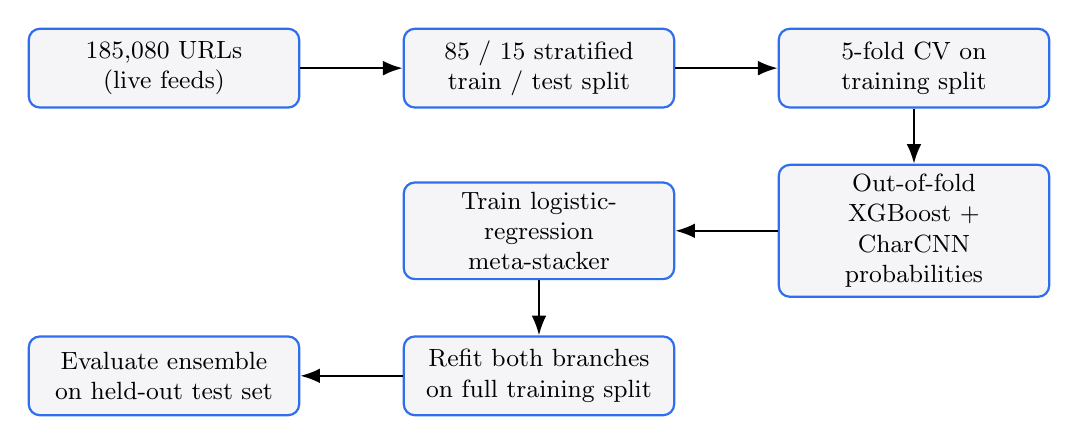
\begin{tikzpicture}[
  node distance=0.7cm and 1.3cm,
  box/.style={rectangle, rounded corners, draw=accentblue, thick, fill=lightgray,
    text width=3.2cm, align=center, minimum height=1cm, font=\small},
  arr/.style={-{Latex[length=2.5mm]}, thick}
]
\node[box] (data) {185{,}080 URLs\\(live feeds)};
\node[box, right=of data] (split) {85 / 15 stratified\\train / test split};
\node[box, right=of split] (kfold) {5-fold CV on\\training split};
\node[box, below=of kfold] (oof) {Out-of-fold\\XGBoost + CharCNN\\probabilities};
\node[box, left=of oof] (meta) {Train logistic-\\regression\\meta-stacker};
\node[box, below=of meta] (refit) {Refit both branches\\on full training split};
\node[box, left=of refit] (eval) {Evaluate ensemble\\on held-out test set};

\draw[arr] (data) -- (split);
\draw[arr] (split) -- (kfold);
\draw[arr] (kfold) -- (oof);
\draw[arr] (oof) -- (meta);
\draw[arr] (meta) -- (refit);
\draw[arr] (refit) -- (eval);
\end{tikzpicture}
\caption{Training and stacking pipeline (\url{pipeline/train.py}), from raw data to held-out evaluation.}
\label{fig:training}
\end{figure}

\section{GPU Acceleration}
The CharCNN branch is trained on an NVIDIA GPU (CUDA 12.4 build of PyTorch). Moving
training from CPU to GPU was necessary purely for iteration speed: on this
dataset size, GPU training reduced full pipeline training time (feature extraction +
5-fold CV for both branches + final refits) from an estimated 10--15 minutes on CPU
to under 5 minutes end-to-end.

\chapter{Results}

\section{Held-Out Test Set Performance}
Table~\ref{tab:results} reports accuracy and ROC-AUC for each branch individually
and for the final stacked ensemble, all measured on the 27{,}762-URL held-out test
set that took no part in training, cross-validation, or threshold selection.

\begin{table}[H]
\centering
\begin{tabular}{lrr}
\toprule
\textbf{Model} & \textbf{Accuracy} & \textbf{ROC-AUC} \\
\midrule
XGBoost (lexical features only) & 97.71\% & 0.9976 \\
CharCNN (raw URL only) & 99.13\% & 0.9997 \\
\textbf{Hybrid ensemble (stacked)} & \textbf{99.30\%} & \textbf{0.9996} \\
\bottomrule
\end{tabular}
\caption{Held-out test set performance, 27{,}762 URLs.}
\label{tab:results}
\end{table}

The stacked ensemble outperforms either branch alone on accuracy, confirming that the
two branches make partially independent errors that the meta-stacker can correct for.

\section{Most Important Lexical Features}
Table~\ref{tab:features} lists the ten most important features for the XGBoost
branch, by Gini importance. Subdomain count dominates, consistent with the
well-established pattern of phishing kits using long, multi-level subdomains
(often on compromised or free-hosting infrastructure) to bury the true domain from a
casual glance at the URL.

\begin{table}[H]
\centering
\begin{tabular}{lr}
\toprule
\textbf{Feature} & \textbf{Importance} \\
\midrule
Number of subdomains & 0.333 \\
Longest path/word segment length & 0.080 \\
Path length & 0.060 \\
Suspicious TLD flag & 0.058 \\
HTTPS usage & 0.043 \\
Path depth & 0.039 \\
Hostname length & 0.035 \\
Number of hyphens & 0.033 \\
Presence of \texttt{@} symbol & 0.028 \\
Number of dots & 0.026 \\
\bottomrule
\end{tabular}
\caption{Top-10 lexical features by XGBoost Gini importance.}
\label{tab:features}
\end{table}

\section{Adversarial and Sanity Test Suite}
Beyond the held-out statistical test set, a hand-built suite of 14 URLs was used to
sanity-check behavior on cases a random held-out sample might not emphasize --- well
known legitimate sites with unusual path conventions, obvious phishing patterns, and
one adversarial look-alike-domain construction. The final pipeline (including the
allow-list safeguard) classified all 14 correctly, summarized in
Table~\ref{tab:adversarial}.

\begin{table}[H]
\centering
\small
\begin{tabular}{p{7.9cm}p{1.8cm}p{1.8cm}}
\toprule
\textbf{URL} & \textbf{Expected} & \textbf{Predicted} \\
\midrule
\texttt{google.com} & Legit & Legit \\
\texttt{github.com/anthropics/claude-code} & Legit & Legit \\
\texttt{gitlab.com/gitlab-org/gitlab} & Legit & Legit \\
\texttt{en.wikipedia.org/wiki/Phishing} & Legit & Legit \\
\texttt{youtube.com/watch?v=\ldots} & Legit & Legit \\
\texttt{stackoverflow.com/questions/\ldots} & Legit & Legit \\
\texttt{amazon.com/dp/\ldots} & Legit & Legit \\
\texttt{npmjs.com/package/react} & Legit & Legit \\
\texttt{paypa1-secure-login.tk/verify/account} & Phishing & Phishing \\
\texttt{192.168.1.1/login.php} & Phishing & Phishing \\
\texttt{coincommunity-ta.netlify.app} & Phishing & Phishing \\
\texttt{microsoft-support-verify.xyz/\ldots} & Phishing & Phishing \\
\texttt{secure-appleid-verify.com/signin} & Phishing & Phishing \\
\texttt{github.com.verify-login.tk/\ldots} (adversarial) & Phishing & Phishing \\
\bottomrule
\end{tabular}
\caption{Hand-built sanity/adversarial test suite -- 14/14 correct on the final pipeline.}
\label{tab:adversarial}
\end{table}

The last row is the most important: it embeds the trusted string
\texttt{github.com} as a \emph{subdomain} of an attacker-controlled domain
(\texttt{verify-login.tk}). The allow-list correctly does \emph{not} fire here,
because it matches on the properly-parsed registered domain rather than a substring
search -- confirming the safeguard cannot be trivially bypassed.

\section{A Debugging Case Study: The Path-Complexity Bug}
The first fully-trained version of this pipeline reached 99.02\% held-out accuracy,
yet flagged \url{https://github.com/anthropics/claude-code} as 99.66\% likely to
be phishing. Investigating the individual lexical features for that URL showed
nothing suspicious (HTTPS used, no IP host, no suspicious TLD, no brand
typosquatting) -- yet the XGBoost branch alone assigned it a phishing probability of
1.0. The root cause, traced by inspecting the training data generator, was that the
synthetic legitimate URLs used only about 20 fixed, trivially simple path templates,
while real phishing URLs are naturally far more path-diverse; the model had learned
``complex path'' as a proxy for phishing rather than any of the intended features.
Section~7.2 describes the fix (richer, realistic synthetic path generation), and
Section~6.4 describes the complementary allow-list safeguard added once it became
clear that no amount of synthetic diversity alone could realistically cover every
legitimate path convention on the internet. This episode is included here
deliberately: it is a useful illustration of why held-out accuracy alone is not
sufficient validation, and why targeted, hypothesis-driven spot-checks against
real-world URLs remain an essential part of evaluating any URL classifier.

\chapter{Web Application}

\section{Overview}
The trained pipeline is served through a Flask web application
(\texttt{app.py}) exposing a single page: a URL input box and, on submission, a
verdict panel showing the overall phishing probability, the detected risk factors
(in plain language, not raw feature names), and a transparent breakdown of each
branch's individual score.

\screenshot{ml_homepage.png}{0.62}{The Phishing URL Checker home page.}

\screenshot{ml_phishing_result.png}{0.62}{Result for a phishing test URL (\texttt{paypa1-secure-login.tk}): 99.8\% phishing risk, with the six triggered risk factors (suspicious TLD, missing HTTPS, hyphenated domain, high URL entropy, near-miss brand typo, credential/urgency keywords) and the individual XGBoost (96.4\%) and CharCNN (99.9\%) branch scores shown transparently.}

\screenshot{ml_legit_result.png}{0.62}{Result for a legitimate URL (\texttt{wikipedia.org}): 99.76\% safe, with no risk factors triggered and both branch scores low.}

\section{Design Rationale}
Showing the two branch scores separately (rather than only the final blended
verdict) was a deliberate transparency choice: a security analyst reviewing a
borderline case can see \emph{why} the model reached its conclusion -- whether the
structural features or the raw-character model drove the decision -- rather than
being handed an opaque single number.

\chapter{Conclusion and Future Work}

\section{Summary}
This project delivers two complementary, independently useful systems: a set of
realistic, self-contained phishing simulations with built-in measurement and
immediate self-disclosure, suitable for running internal security-awareness
exercises; and a hybrid ML/DL phishing-URL classifier that improves on a
single-model baseline by combining hand-engineered lexical features with a
learned character-level representation, trained on live rather than static data,
and hardened with an explicit, auditable allow-list safeguard. The final system
reaches 99.3\% accuracy (ROC-AUC 0.9996) on a held-out test set of 27{,}762 URLs
never seen during training, and passes a 14-case hand-built adversarial sanity
suite including a subdomain-impersonation attack against its own safeguard.

\section{Future Work}
\begin{itemize}[leftmargin=1.4em]
  \item Extend the simulation suite with additional pretexts (spear-phishing using
  scraped public employee data, vishing call scripts) and multi-organization
  campaign management in the dashboard.
  \item Periodically retrain the detection pipeline on refreshed PhishTank/Umbrella
  snapshots to track drifting attacker tooling over time, and monitor for
  distributional drift in production.
  \item Explore replacing the fixed 100-word synthetic-path vocabulary with paths
  sampled from a real, licensed web crawl, to further close the residual gap between
  synthetic and real-world legitimate URL diversity.
  \item Add explainability tooling (e.g.\ SHAP values) for the XGBoost branch to
  give security analysts a per-prediction feature attribution, beyond the current
  static global importance ranking.
\end{itemize}

\end{document}
